% 例 2：A(1,2), B(4,1), C(5,4)，等腰直角三角形（B 为直角顶点）
\documentclass[tikz,border=4pt]{standalone}
\usepackage{ctex}
\usepackage{amsmath}
\usetikzlibrary{calc}
\begin{document}
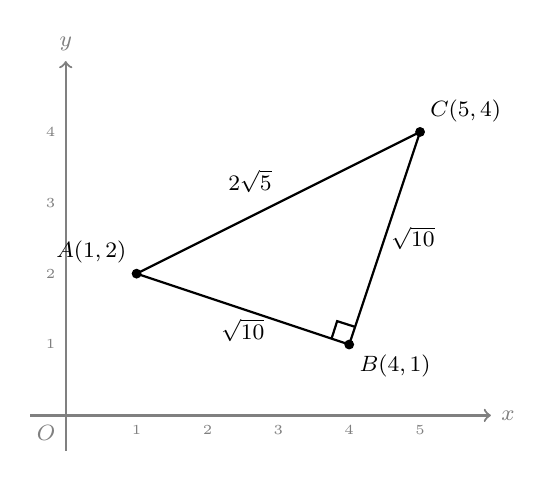
\begin{tikzpicture}[thick, scale=0.9]
  \draw[->, gray] (-0.5,0) -- (6,0) node[right, font=\footnotesize] {$x$};
  \draw[->, gray] (0,-0.5) -- (0,5) node[above, font=\footnotesize] {$y$};
  \foreach \i in {1,...,5} \node[font=\tiny, below, gray] at (\i,0) {$\i$};
  \foreach \j in {1,...,4} \node[font=\tiny, left, gray] at (0,\j) {$\j$};
  \node[font=\footnotesize, below left, gray] at (0,0) {$O$};
  \coordinate (A) at (1,2);
  \coordinate (B) at (4,1);
  \coordinate (C) at (5,4);
  \draw[thick] (A) -- (B) -- (C) -- cycle;
  \filldraw (A) circle (1.5pt) node[above left, font=\footnotesize] {$A(1,2)$};
  \filldraw (B) circle (1.5pt) node[below right, font=\footnotesize] {$B(4,1)$};
  \filldraw (C) circle (1.5pt) node[above right, font=\footnotesize] {$C(5,4)$};
  % 边长标注
  \node[font=\footnotesize] at ($(A)!0.5!(B) + (0,-0.3)$) {$\sqrt{10}$};
  \node[font=\footnotesize] at ($(B)!0.5!(C) + (0.4,0)$) {$\sqrt{10}$};
  \node[font=\footnotesize] at ($(A)!0.5!(C) + (-0.4,0.3)$) {$2\sqrt{5}$};
  % 直角标记于 B
  % AB 方向 (-3,1)/sqrt(10), BC 方向 (1,3)/sqrt(10)；它们垂直
  \draw (4-0.25, 1+0.08) -- (4-0.17, 1+0.33) -- (4+0.08, 1+0.25);
\end{tikzpicture}
\end{document}
